\input{header}
\graphicspath{{images/}}

\usepackage[
	colorlinks=true,
	urlcolor=blue,
	linkcolor=black
]{hyperref}

\title{Robot Motion Planning}
\author{\url{https://github.com/MichaelGrupp/RobotMotionPlanning_summary} \\ TU München - Fakultät für Informatik - Robotics, Cognition, Intelligence}
\date{\the\year}


\begin{document}

\maketitle

\begin{multicols*}{2}  %2 columns, uncomment \end{multicols*} too if you want single column


\section{Introduction}
The main problem is to find a path from one position or configuration to another, without colliding with the environment. Planning algorithms can be rated regarding different aspects.

Performance metrics for path planning algorithms: 
\begin{itemize}
	\item path length
	\item execution speed
	\item planning time
	\item safety (distance to obstacles)
	\item robustness to disturbances
	\item probability of success
\end{itemize}

\section{Configuration Space}

A configuration describes the state of a robot as a combination of different configurations of its degrees of freedom. For example, a mobile robot moves in directions $x,y$ and can turn its yaw heading $\theta$ - a configuration of this robot could be $c = (1,3,30^\circ)^\mathrm{T}$ The configuration space (\textit{C-space}) is the space of all possible configurations, that a robot can have in a certain workspace.

The dimension of the C-space is equal to the degrees of freedom of the robot (minimum number of parameters needed to specify the configuration). Because there can also be angles in the topology of the C-space, it is usually not a cartesian space (e.g. $2\pi = 4\pi$, cyclic repetition along angle axis).

A non-holonomic robot is a robot, that cannot move freely on the
configuration space manifold because it is constrained in some way. For example, a car cannot drive sideways.

\subsection{Point Representation}
In order to determine the C-space / free space of configurations, a point representation can be useful. For example, if we have a circular robot with radius $r$ and some obstacles in the workspace, the robot can be reduced to a point if the obstacle boundaries are "blown up" by the radius of the robot. In other words, to get a smaller representation of the robot without changing the properties of the workspace, the obstacles have to get bigger. 

$\Rightarrow$ Minkowski sum algorithm


\includegraphics[width=0.3\columnwidth]{pointrep}

\section{Bug Algorithms}
Bug algorithms are simple strategies that use local knowledge (e.g. from sensor input) instead of global knowledge.

\textbf{Assumptions: }
\begin{itemize}
	\item robot is a point in a plane
	\item contact sensor to detect obstacle boundaries
\end{itemize}

\textbf{Basic idea:} move on a straight line towards goal and follow the boundaries around obstacles

\subsection{Bug1}
\begin{enumerate}
	\item move towards goal on the \textit{m-line} connecting $q_{start}$ and $q_{goal}$
	\item if an obstacle is detected at a hit-point $q^H_i$, move left (or right) along its boundary until you return to $q^H_i$ again
	\item while circumnavigating the obstacle, calculate and save the distance to the goal at any coordinate
	\item determine the closest point to the goal on the boundary and use it as a leave point $q^L_i$
	\item from $q^L_i$, go straight to the goal again on the m-line $q^L_i$ and $q_{goal}$
	\item if the line that connects $q^L_i$ and the goal intersects the current obstacle, then there is no path to the goal
\end{enumerate}
\includegraphics[width=0.6\columnwidth]{bug1.png}



\subsection{Bug2}
The m-line of Bug2 does not change and it connects $q_{start}$ and $q_{goal}$.
\begin{enumerate}
	\item move towards goal on the \textit{m-line} connecting $q_{start}$ and $q_{goal}$
	\item if an obstacle is detected at a hit-point $q^H_i$, move left (or right) along its boundary
	\item if a point on the m-line is found and it is closer to the goal than $q^H_i$, use it as a leave point $q^L_i$
	\item from $q^L_i$, go straight to the goal again on the m-line
	\item if the robot re-encounters the original departure point $q^H_i$ from the m-line, then there is no path to the goal
\end{enumerate}
\includegraphics[width=0.8\columnwidth]{bug2.png}

\subsection{Tangent Bug}
The robot is equipped with a (finite-range) radial distance sensor. If an obstacle is encountered within the range of the sensor, the robot changes its direction tangentially to the border of the obstacle.

\section{Roadmapping with Exact Knowledge}
The basic idea of a roadmap is to "capture the connectivity of the free space in a network of one-dimensional curves" (\textit{Latombe}). Using this network, paths can be calculated using graph-search algorithms, for example. The advantage of a roadmap is that it only has to be constructed once if the topology of the workspace (i.e. obstacle positions) does not change. On the other hand, roadmaps can be not very efficient in dynamic environments.

\subsection{Visibility Graph}
The visibility graph applies to 2-dimensional configuration spaces with polygonal obstacles. The graph's nodes are the initial configuration $q_{init}$ (start) and the goal configuration $q_{goal}$, as well as the vertices/edges of the obstacles. Two nodes are connected with a straight line if the connecting line does not intersect with an obstacle.
\includegraphics[width=0.8\columnwidth]{visGraph}

Unfortunately, the visibility graph can contain useless edges. This can be resolved by constructing the reduced visibility graph, where only edges are kept that are separating or supporting lines between two obstacles. 

\includegraphics[width=0.7\columnwidth]{visGraph2}

\subsection{Voronoi Diagram}
The goal of the Voronoi diagram is to find paths that maximize the distance to the obstacles. Therefore, the roadmap lines can be curved.

\includegraphics[width=0.7\columnwidth]{voronoi}

To construct the Voronoi diagram, one can use the Brushfire algorithm, which calculates a distance map on a grid:
\begin{itemize}
	\item grid initialization: free space = 0, obstacle space = 1
	\item for each point in the grid, assign the distance to the closest obstacle point
	\item every point, where the distance to two (or more) different obstacles is the same, lies on the Voronoi diagram
\end{itemize}
("wavefront from obstacles, Voronoi diagram where two wavefronts meet")

\subsection{Cell Decomposition}
Main idea: decompose the free space into simple cells and represent the connectivity of the free space $\mathcal{F}$ by the adjacency of these cells. It is called an exact cell decomposition if the union of all cells is exactly $\mathcal{F}$, meaning there is no overlap between cells. 

The shape of the cells can be triangles, trapezoids, ...

\subsubsection{Trapezoidal Decomposition}
Free space is decomposed into trapezoids and triangles. Then, the adjacency graph of the cells is calculated.
\includegraphics[width=0.7\columnwidth]{cell}

\subsubsection{Boustrophedon Decomposition}
Points on the obstacles, from which a separating line can be drawn in the upper and lower direction are called critical points. Then, an exhaustive walk through the critical points is performed in order to obtain a connectivity graph.
\includegraphics[width=\columnwidth]{boustro}

\subsection{Potential Field Method}
The C-space is turned into a potential field, where the obstacles are surrounded by a repulsive field and the goal location by an attractive field. To navigate, the robot applies a force proportional to the negative gradient of the field - this is called gradient descent. 

The advantage of potential field methods is that they are easy to compute. On the other hand, they can suffer from local minima (where robot gets stuck), and they don't consider dynamic constraints in their initial form (forces can be too high).

\includegraphics[width=0.6\columnwidth]{potential}


\section{Roadmapping with Random Sampling}
Instead of looking at the whole space, sampling based methods are usually more efficient because they only require point-wise evaluations. They are probabilistically complete, meaning the probability that they will produce a solution approaches 1 as more time is spent. However, they are not as robust as methods with full knowledge of the space and cannot determine if there is no solution to the path planning problem.

\subsection{Multi-Query}
A multiple query approach tries to capture the connectivity of the free space as good as possible, such that multiple, different queries for paths can be answered very fast. In other words: create a roadmap that is suitable for as many use cases as possible.

\subsubsection{PRM - Probabilistic Roadmaps}
Basic steps for constructing PRMs:
\begin{enumerate}
	\item sample vertices and keep vertices that do not lie on an obstacle
	\item find neighbour vertices
		\subitem k-nearest neighbour or
		\subitem neighbours within a specified radius
	\item connect neighbouring vertices with edges (lines) (and check for collisions on connecting line using e.g. discretized line search)
	\item add vertices and edges until roadmap is dense
enough
\end{enumerate}
\includegraphics[width=\columnwidth]{PRM}
\textbf{Drawbacks: } PRMs don't perform well when there are narrow passages.

\subsubsection{OBPRM - Obstacle-Based PRM}
Obstacle-based PRMs are constructed by sampling only close to obstacles. During sampling, the first goal is to find a point that lies inside an obstacle. Then, another point is sampled at an arbitrary distance to the first point. Using step-wise approximation, a point sufficiently close to the obstacle border is searched.
\includegraphics[width=\columnwidth]{OBPRM}

\subsection{Single-Query}
Single query planners try to solve a single query as fast as possible, without trying to cover the whole free space.

\subsubsection{Weighted Randomized Tree Expansion}

\begin{enumerate}
	\item expand trees from start and goal
	\item pick a node with probability $1/w(x)$, with $w(x)$ being the amount of neighbors within radius (~ measurement for exploration around $x$)
	\item sample $k$ points ($y_1, ..., y_k$) around $x$
	\item add $y_i$ to the tree if
	\begin{enumerate}
		\item $1/w(y_i) > 1/w(x)$
		\item $y_i$ is collision free
		\item $y_i$ can see $x$
	\end{enumerate}
	\item if a pair of nodes from start tree and goal tree are close and can see each other, then connect them and terminate
\end{enumerate}

\begin{minipage}[t]{.5\columnwidth}
	\raggedright
	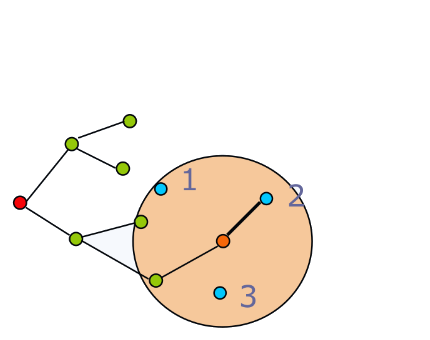
\includegraphics[width=\columnwidth]{weighted_expansion_2.png}
\end{minipage}%
\begin{minipage}[t]{.5\columnwidth}
	\raggedleft
	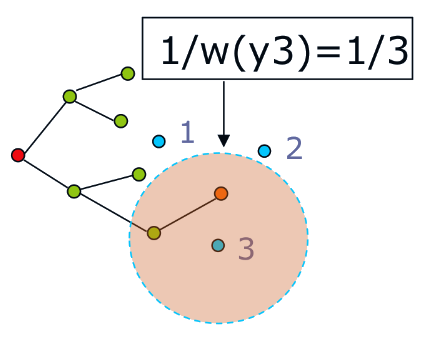
\includegraphics[width=\columnwidth]{weighted_expansion_1.png}
\end{minipage}


\subsubsection{RRT - Rapidly Exploring Random Trees}
\begin{enumerate}
	\item pick $q_{start}$ as the first node
	\item pick a random target location (every $n$-th
iteration, choose $q_{goal}$) \label{targetRRT}
	\item find closest vertex in roadmap
	\item extend this vertex towards target location
	\item repeat steps until $q_{goal}$ is reached
\end{enumerate}
\textit{Note to point \ref{targetRRT}:} $q_{goal}$ is not chosen as target every time, because this would possibly lead the tree into an obstacle instead of exploring the free space.

For faster execution, the tree can be grown from both $q_{start}$ and $q_{goal}$

\includegraphics[width=0.8\columnwidth]{RRT}


\subsection{How To Sample}
\begin{itemize}
	\item unit line, square, cube: pick a random number $r\in [0,1]$ for each dimension
	\item intervals shifted by $c$ \& scaled by $s$: $sr+c, ~ r\in [0,1]$ 
	\item circle: pick an angle $\theta \in [0, 2\pi]$ for a unit sphere uniformly at random
	\item rotations: depends on representation, in axis-angle notation the axis and the angle are sampled separately
\end{itemize}

\subsection{Coverage, Connectivity, $\epsilon, \alpha, \beta$ - Expansiveness}
A PRM has good coverage if the milestones are distributed in such a way that (almost) any point in the free C-space can be connected to one milestone via a straight line. Also, the connectivity should be good, meaning that every milestone should be reachable from any other milestone. Especially with narrow passages, the connectivity can be hard to capture.

\includegraphics[width=\columnwidth]{coverage}

The coverage and connectivity are characterized by the expansiveness of the space (given by $\epsilon$, $\alpha$, $\beta$).

\textbf{Definition from Hsu's paper:} A free space $F$ is ($\alpha$, $\beta$, $\epsilon$)-expansive, if it satisfies these conditions: 
\begin{enumerate}
	\item $\mu (V(p))  \geq \epsilon , ~~ \forall p \in F$ \\
	$\Rightarrow$ each point p must see at least a $\epsilon$ fraction of the free space F $\rightarrow$ F is $\epsilon$-good
	\item $\beta-\mathrm{lookout}(S) = \{q\in S ~~|~~ \mu(V(q)\textbackslash S) \geq \beta \cdot \mu(F\textbackslash S)\} $ \\
	$\Rightarrow$ for any $S \subseteq F$, the $\beta-\mathrm{lookout}(S)$ is defined as the subset of points $p$ that can see at least a $\beta$-fraction of the complementary space of $S$ ($\equiv F\textbackslash S$). $\alpha$ is then defined as the relative volume of these points $p$ to $S$: $\frac{\mu(\beta-\mathrm{lookout}(S))}{\mu(S)}$
\end{enumerate}

with $\epsilon, \alpha, \beta \in \ (0,1]$, $V(\cdot)$ as the set of visible points of a point and $\mu(\cdot)$ denoting the volume of a set of points.

~\\
\textbf{Burschka-Style}:
\begin{enumerate}
	\item let $F$ be the free space (set of points); $\mu(G)$ the volume/ area of some set G; $reach(x)$ the space ($\subseteq F$) that can be seen from some point $x$; $reach(G)$ the space that can be seen from any point in a set $G$
	\item find point $x \in F$ with smallest $\mu(reach(x))$
	\item $S = reach(x)$
	\item $\epsilon = \frac{\mu(S)}{\mu(F)}$
	\item choose some set $Z \subseteq S$ that can reach a lot and has an easy to calculate area
	\item $\alpha = \frac{\mu(Z)}{\mu(S)}$
	\item $\beta = \frac{\mu(reach(Z) \setminus S)}{\mu(F \setminus S)}$ (not really according to the definition, but best way to do it in the exam)
	\item the goal is to keep $\alpha$ and $\beta$ balanced
\end{enumerate}

Using these values, the number n of samples that is needed for a good connectivity can be calculated:
\[ n= \frac{8 \ln (\frac{8}{\epsilon\alpha\gamma})}{\epsilon\alpha} + \frac{3}{\beta} \,, \] 
where $1-\gamma$ measures the probability that the uniformly sampled milestones have the correct connectivity ($\gamma \in [0,1]$).

\subsection{Path and Map Smoothing}
The paths obtained by random sampling techniques are not necessarily the most efficient paths. Path smoothing techniques are used to optimize the path for length, energy, distance to obstacles etc. 

To grow the distance to obstacles, the map can be smoothed by itself before planning. For example, a 2D-convolution with a Gaussian filter kernel leads to a non-zero probability distribution around the edges of the obstacles (edge smoothing).

\includegraphics[width=0.6\columnwidth]{mapGaussian}
 
After planning, the path can be optimized, too. For example, the number of "zick-zacks" of the path can be reduced by connecting pairs of nodes that are in sight of each other with straight lines. Furthermore, the path can be also optimized regarding the energy efficiency for the robot using some non-linear optimization technique to minimize the energy cost.

\includegraphics[width=0.9\columnwidth]{pathSmooth}

\section{Probabilistic Robotics}

\subsection{Kalman Filter}

The basic idea of a Kalman filter is that you interpret your robots state as a normal (gaussian) distribution with mean and variance. Furthermore you model your sensors with white noise (gaussian, zero-mean).

\paragraph{predict/ time update}

\begin{align}
	&\text{mean} && \hat{x}_{k+1}^- = A \hat{x}_{k} + B u_k  \\
	&\text{covariance } \textcolor{gray}{\sigma_3^2 = \sigma_1^2 + \sigma_2^2} && P_{k+1}^- = A P_k A^\top + Q 
\end{align}

\paragraph{correct/ measurement update}

\begin{align}
	&\text{Kalman Gain} && K_k = P_k^- H^\top (H P_k^- H^\top + R)^{-1} \\
	&\text{mean} && \hat{x}_k = \hat{x}_k^- + K_k (z_k - H \hat{x}_k^-) \\
	&\text{covariance } \textcolor{gray}{\sigma_3^2 = \frac{\sigma_1^2  \sigma_2^2}{\sigma_1^2 + \sigma_2^2}}  && P_k = (I - K_k H) P_k^-
\end{align}

\paragraph{with}

\begin{flalign*}
	\hat{x} & \text{ - state estimate mean} & \\
	\hat{x}^- & \text{ - predicted state estimate mean} & \\
	A & \text{ - state propagation/ transfer function} & \\
	u & \text{ - control input} & \\
	B & \text{ - mapping from control space to state space} & \\
	P & \text{ - state covariance} & \\
	Q & \text{ - process noise/ uncertainty covariance} & \\
	K & \text{ - Kalman Gain} & \\
	R & \text{ - measurement noise covariance} & \\
	z & \text{ - measurement} &
\end{flalign*}

\paragraph{Observability}

\begin{align*}
O = \begin{bmatrix} H \\ HA^1 \\ \vdots  \\ HA^{n-1} \end{bmatrix}
\end{align*}

The system is observable if $rank(O) = n$ ($O$ has $n$ linearly independent rows).

\subsection{Extended Kalman Filter}
The (first order) EKF allows to use non-linear system models for Kalman filtering. The EKF adapts techniques from calculus, namely multivariate Taylor Series expansions, to linearize a model about a working point. 

\paragraph{predict/ time update}

\begin{align}
	&\text{mean} && \hat{x}_{k+1}^- = f(\hat{x}_k, u_k, 0)  \\
	&\text{covariance } && P_{k+1}^- = A_{k+1} P_k A_{k+1}^\top + W_{k+1} Q W_{k+1}^\top 
\end{align}

\paragraph{correct/ measurement update}

\begin{align}
	&\text{Kalman Gain} && K_k = P_k^- H_k^\top (H_k P_k^- H_k^\top + V_k R V_k^\top)^{-1} \\
	&\text{mean} && \hat{x}_k = \hat{x}_k^- + K_k (z_k - h(\hat{x}_k^-, 0)) \\
	&\text{covariance }  && P_k = (I - K_k H_k) P_k^-
\end{align}

\paragraph{with}

\begin{flalign*}
	f(x, u, n) & \text{ - state transfer function} & \\
	n & \text{ - process noise} & \\
	A & \text{ - Jacobian of $f$ with respect to $x$} & \\
	W & \text{ - Jacobian of $f$ with respect to $n$} & \\
	h(x, v) & \text{ - mapping from state space to measurement space} & \\
	v & \text{ - measurement noise} & \\
	H & \text{ - Jacobian of $h$ with respect to $x$} & \\
	V & \text{ - Jacobian of $h$ with respect to $v$} &
\end{flalign*}

\subsection{Unscented Kalman Filter}
Instead of using first order approximations of the Taylor series (EKF), the unscented filter extends to the second (or higher) order approximations. EKF may cause significant error for highly nonlinear systems because of the propagation of uncertainty through the nonlinear system. However, higher order unscented EKFs tend to only provide performance benefits when the measurement noise is small.

The idea is to produce several sampling points (Sigma Points) from the current state and noise distributions. Then, propagating these points through the nonlinear map to get more accurate estimation of the mean and covariance of the mapping results. In this way, it avoids the need to calculate the Jacobian, hence incurs only the similar computation load as the EKF.

\td{Martin: The indices in the slides seemed mixed up. I hope I corrected them right. I also changed the notation so it is similar to KF and EKF.}

\paragraph{init}

\setlength{\belowdisplayskip}{0pt}
\setlength{\abovedisplayskip}{0pt}

\begin{align}
&\text{mean vector} && \hat{x}_{k-1}^a = \begin{bmatrix}{x}_{k-1}^\top & 0 & 0 \end{bmatrix}^\top \\
\intertext{\small contains mean values of state ($x$), process noise ($v$) and measurement noise ($n$)}
&\text{covariance matrix }  && P_{k-1}^a = \begin{bmatrix}P_{k-1} & 0 & 0 \\ 0 & Q & 0 \\ 0 & 0 & R\end{bmatrix} 
\intertext{\small contains covariances of state, process, and measurement}
&\text{sigma points} && \chi_{k-1}^x = \begin{bmatrix}\hat{x}_{k-1}^x & \hat{x}_{k-1}^x \pm \sqrt{(n_x + \lambda) P_{k-1}^x } \end{bmatrix} \\
\intertext{\small do the same for $v$ and $n$}
&\text{first-order weights} && W_{0}^{(m)} = \frac{\lambda}{n_x + \lambda} \\
&\text{second-order weights} && W_{0}^{(c)} = \frac{\lambda}{n_x + \lambda} + (1 - \alpha^2 + \beta) \\
& && W_i^{(m)} = W_i^{(c)} = \frac{\lambda}{2(n_x + \lambda)} \\
\intertext{\small weighting of sigma points ($x \in \mathbb{R}^{n_x}; i=1,...,2n_x;$)} \nonumber
\end{align}

\paragraph{predict/ time update}

\begin{align}
&\text{sigma points} && \chi_{k}^{x-} = f(\chi_{k-1}^x, \chi_{k-1}^v) \\
&\text{mean state} && \hat{x}_{k}^- = \sum_{i=0}^{2n_x} W_i^{(m)} \chi_{i,k}^{x-} \\
&\text{covariance} && P_k^- = \sum_{i=0}^{2n_x} W_i^{(c)} \begin{bmatrix}\chi_{i,k}^{x-} - \hat{x}_{k}^-\end{bmatrix}\begin{bmatrix}\chi_{i,k}^{x-} - \hat{x}_{k}^-\end{bmatrix}^\top
\end{align}

\paragraph{correct/ measurement update}

\begin{align}
&\text{pred. meas.} && Y_k^- = h(\chi_{k-1}^x, \chi_{k-1}^n) \\
&\text{mean meas.} && \hat{y}_{k}^- = \sum_{i=0}^{2n_x} W_i^{(m)} Y_{i,k}^- \\
&\text{meas. cov.} && P_{y_k y_k} = \sum_{i=0}^{2n_x} W_i^{(c)} \begin{bmatrix}Y_{i,k}^- - \hat{y}_{k}^-\end{bmatrix} \begin{bmatrix}Y_{i,k}^- - \hat{y}_{k}^-\end{bmatrix}^\top \\
&\text{cross cov.} && P_{x_k y_k} = \sum_{i=0}^{2n_x} W_i^{(c)} \begin{bmatrix}\chi_{i,k}^{x-} - \hat{x}_{k}^-\end{bmatrix} \begin{bmatrix}Y_{i,k}^- - \hat{y}_{k}^-\end{bmatrix}^\top \\
&\text{Kalman Gain} && K_k = P_{x_k y_k} P_{y_k y_k}^{-1} \\
&\text{mean state} && \hat{x}_k = \hat{x}_k^- + K_k(y_k - \hat{y}_k^-) \\
&\text{covariance} && P_k = P_k^- - K_k P_{y_k y_k} K_k^\top
\end{align}

\subsection{Bayes Filter}

\td{noch nicht fertig... \\ not yet written...}

\subsection{Particle Filter}
The state representations of the Bayes and Kalman filter are restricted to probability density or Gaussian functions. They cannot model multiple hypotheses in their initial form, for example the uncertainty when a robot could be in one of multiple locations. (Multi-hypothesis KF could do that, but it's only a combination of multiple KFs).

The particle filter uses random sampling techniques together with probabilistic state estimation. The basic principle is:
\begin{enumerate}
	\item if no initial distribution is given, start with a uniform sample distribution
	\item apply motion model \label{pMM}
	\item apply sensor model
	\item resample using Monte Carlo method (sample more into areas where the density of samples (certainty) is higher
	\item repeat from \ref{pMM}
\end{enumerate}



\end{multicols*}
\end{document}
